\section{Generating and Working with IL}

One of BAP's central features is the ability to represent the
semantics of binary code in a simple language called BIL (BAP
Intermediate Language).  This example demonstrates how to lift binary
code to the IL and manipulate it in BAP.  Let's start with the
following assembly file:

\verbatiminput{chap-examples/basic.S}

\subsection{Lifting to the IL}

In this form, the program looks very simple.  Let's see what the BAP
representation of the program shows us.  Compile this file (basic.S)
to an object file with \cmdline{gcc -c basic.S -o basic.o}.  We can
lift this object file with BAP's \cmdline{toil} command: \cmdline{toil
  -bin basic.o -o basic.il}. If you inspect \cmdline{basic.il}, you
should see something like:

\verbatiminput{chap-examples/basic.il}

You can see from this example that BAP IL is much more verbose than
assembly; this is on purpose.  It might make BAP IL a little more
tedious to read, but it makes writing analyses much simpler.  Let's go
through some of the IL line by line to explain what is happening.

\begin{verbatim}
addr 0x0 @asm "add    %eax,%ebx"
label pc_0x0
\end{verbatim}
These two statements mark the beginning of a new assembly instruction.
Note the label for pc\_0x0; any jump to address zero will go to to
this label.

\begin{verbatim}
t:u32 = R_EBX:u32
\end{verbatim}
Here we are saving the original value of \%ebx before it is modified.
This original value will be used when computing flags.

\begin{verbatim}
R_EBX:u32 = R_EBX:u32 + R_EAX:u32
\end{verbatim}
This is the primary computation of the add instruction: adding \%eax
to \%ebx.

\begin{verbatim}
R_CF:bool = R_EBX:u32 < t:u32
\end{verbatim}
Here we explicitly compute the value of the carry flag.  After
executing the add instruction, the carry flag is set if the resulting
value of \%ebx is less than the original value of \%ebx (which is
saved in t).

\begin{verbatim}
R_OF:bool =
  if (R_ECX:u32 & 0x1f:u32) == 0:u32 then R_OF:bool else
  if (R_ECX:u32 & 0x1f:u32) == 1:u32 then high:bool(R_EBX:u32) ^ R_CF:bool
  else unknown "OF <- undefined":bool
\end{verbatim}
Here we are explicitly computing the overflow flag after the shl
instruction.  Note that the IL uses if then else expressions.  Also
note that the the overflow flag can be set to an unknown expression
when the Intel semantics says the flag should be undefined.

\begin{verbatim}
cjmp R_CF:bool, 8:u32, "nocjmp0"
\end{verbatim}
This is a conditional jump.  If the condition (in this case, the carry
flag) evalutes to true, control will transfer to label pc\_0x8.
Otherwise, it will go to the label nocjmp0.

\subsection{Built-in Graphs and Analyses}

We might want to visualize what's going on.  There are several ways to
do this in BAP, including control flow graphs (CFG), control
dependence graphs (CDG), and data dependence graphs (DDG).  These can
be generated with the iltrans tool.  iltrans takes a program as input,
and then applies transformations in a pipeline.  The visualizations we
want require the program to be in Single Static Assignment (SSA) form.
The command \cmdline{iltrans -il basic.il -to-ssa} will do this.  If
we want to print the control flow graph, we can add \cmdline{-pp-ssa
  out.dot} to the end, for \cmdline{iltrans -il basic.il -to-ssa
  -pp-ssa out.dot}. The resulting file out.dot is a file that can be
processed with GraphViz's dot command: \cmdline{dot -Tpdf out.dot -o
  out.pdf}.  The output should look similar to what is shown in
Figure~\ref{fig:cfg}. The CDG and DDG can be generated by using
\cmdline{-pp-ssa-cdg} and \cmdline{-pp-ssa-ddg} respectively. Examples
are shown in Figures~\ref{fig:cdg} and \ref{fig:ddg}.

BAP also has built-in optimizations.  To apply them, simply use the
\cmdline{-ssa-simp} iltrans flag.  If we apply this before producing
the CFG, we can see the IL is greatly simplified: \cmdline{iltrans -il
  basic.il -to-ssa -ssa-simp -pp-ssa out.dot}. This is shown in
Figure~\ref{fig:cfgsimp}.

\begin{figure}[!p]
  \begin{center}
    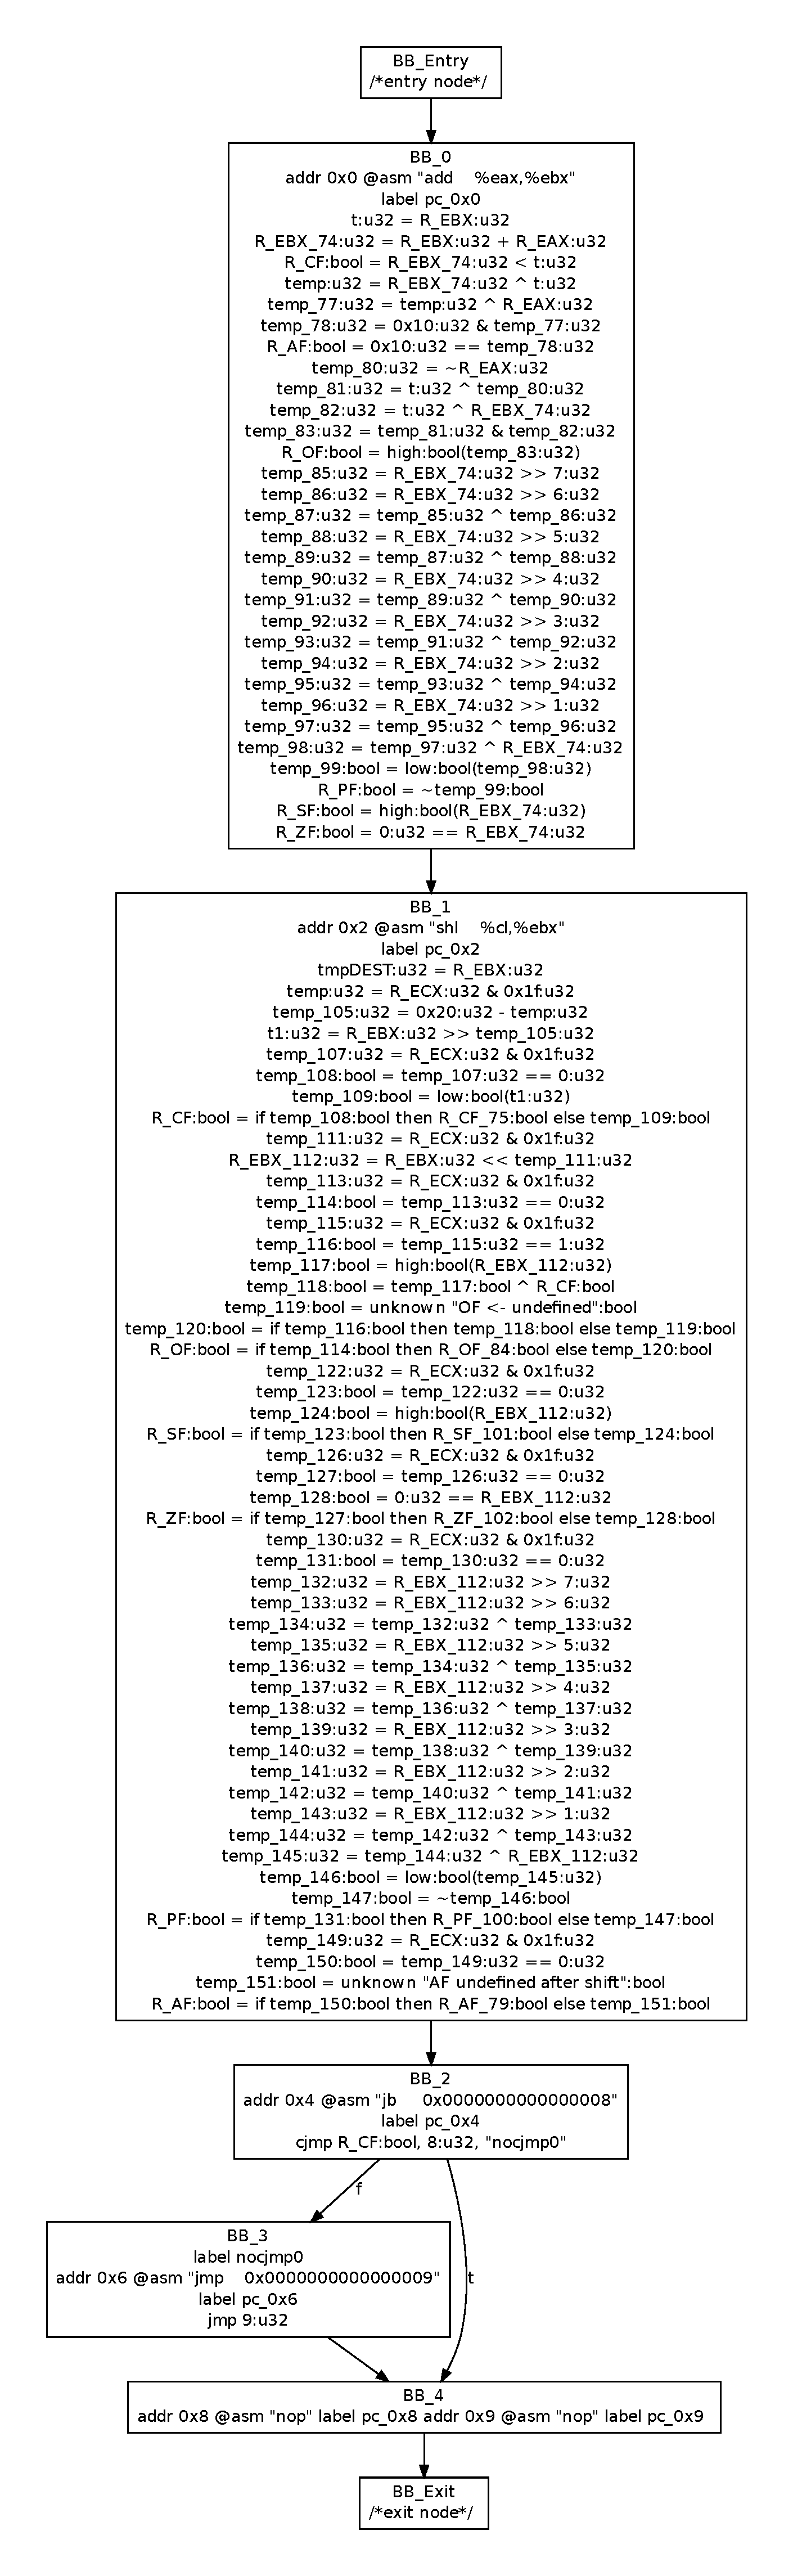
\includegraphics[height=.9\textheight]{chap-examples/cfg.pdf}
  \end{center}
  \caption{Example CFG}
  \label{fig:cfg}
\end{figure}

\begin{figure}[p]
  \begin{center}
    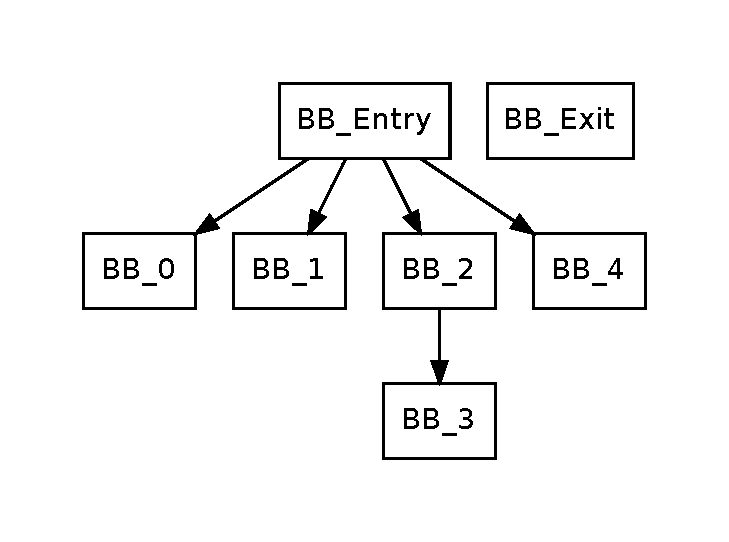
\includegraphics{chap-examples/cdg.pdf}
  \end{center}
  \caption{Example CDG}
  \label{fig:cdg}
\end{figure}

\begin{figure}[p]
  \begin{center}
    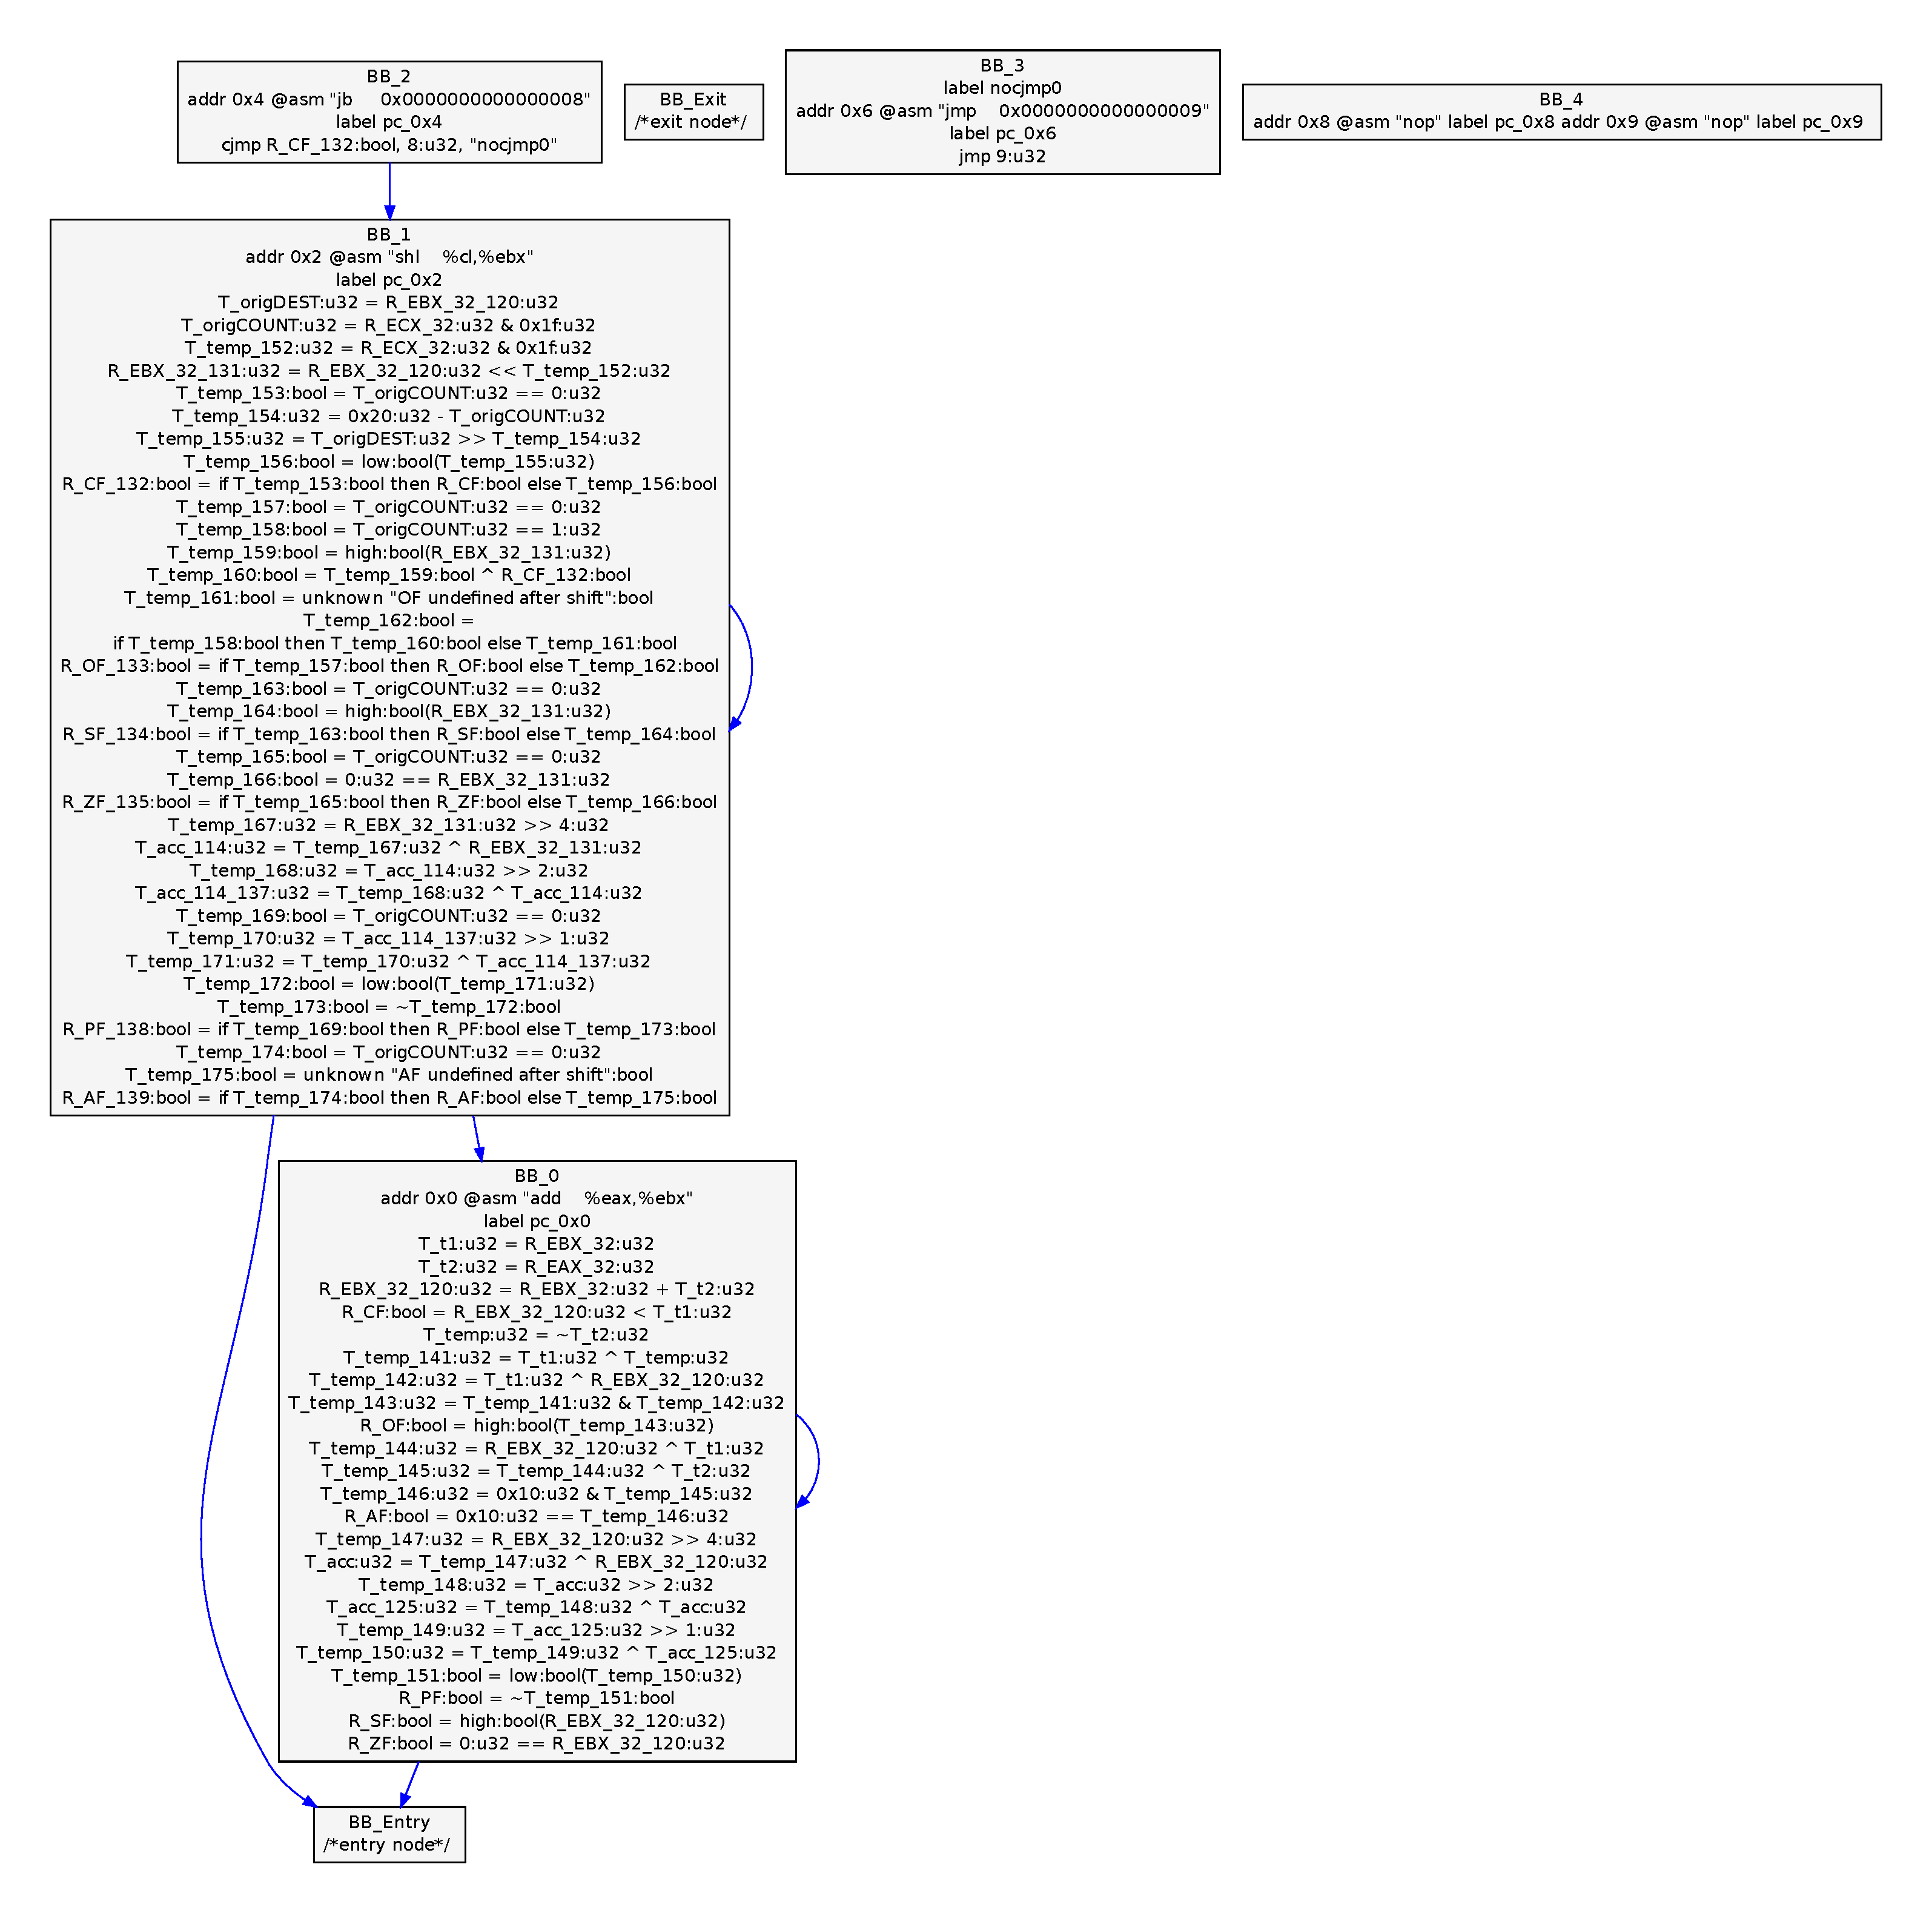
\includegraphics[height=.9\textheight]{chap-examples/ddg.pdf}
  \end{center}
  \caption{Example DDG}
  \label{fig:ddg}
\end{figure}

\begin{figure}[p]
  \begin{center}
    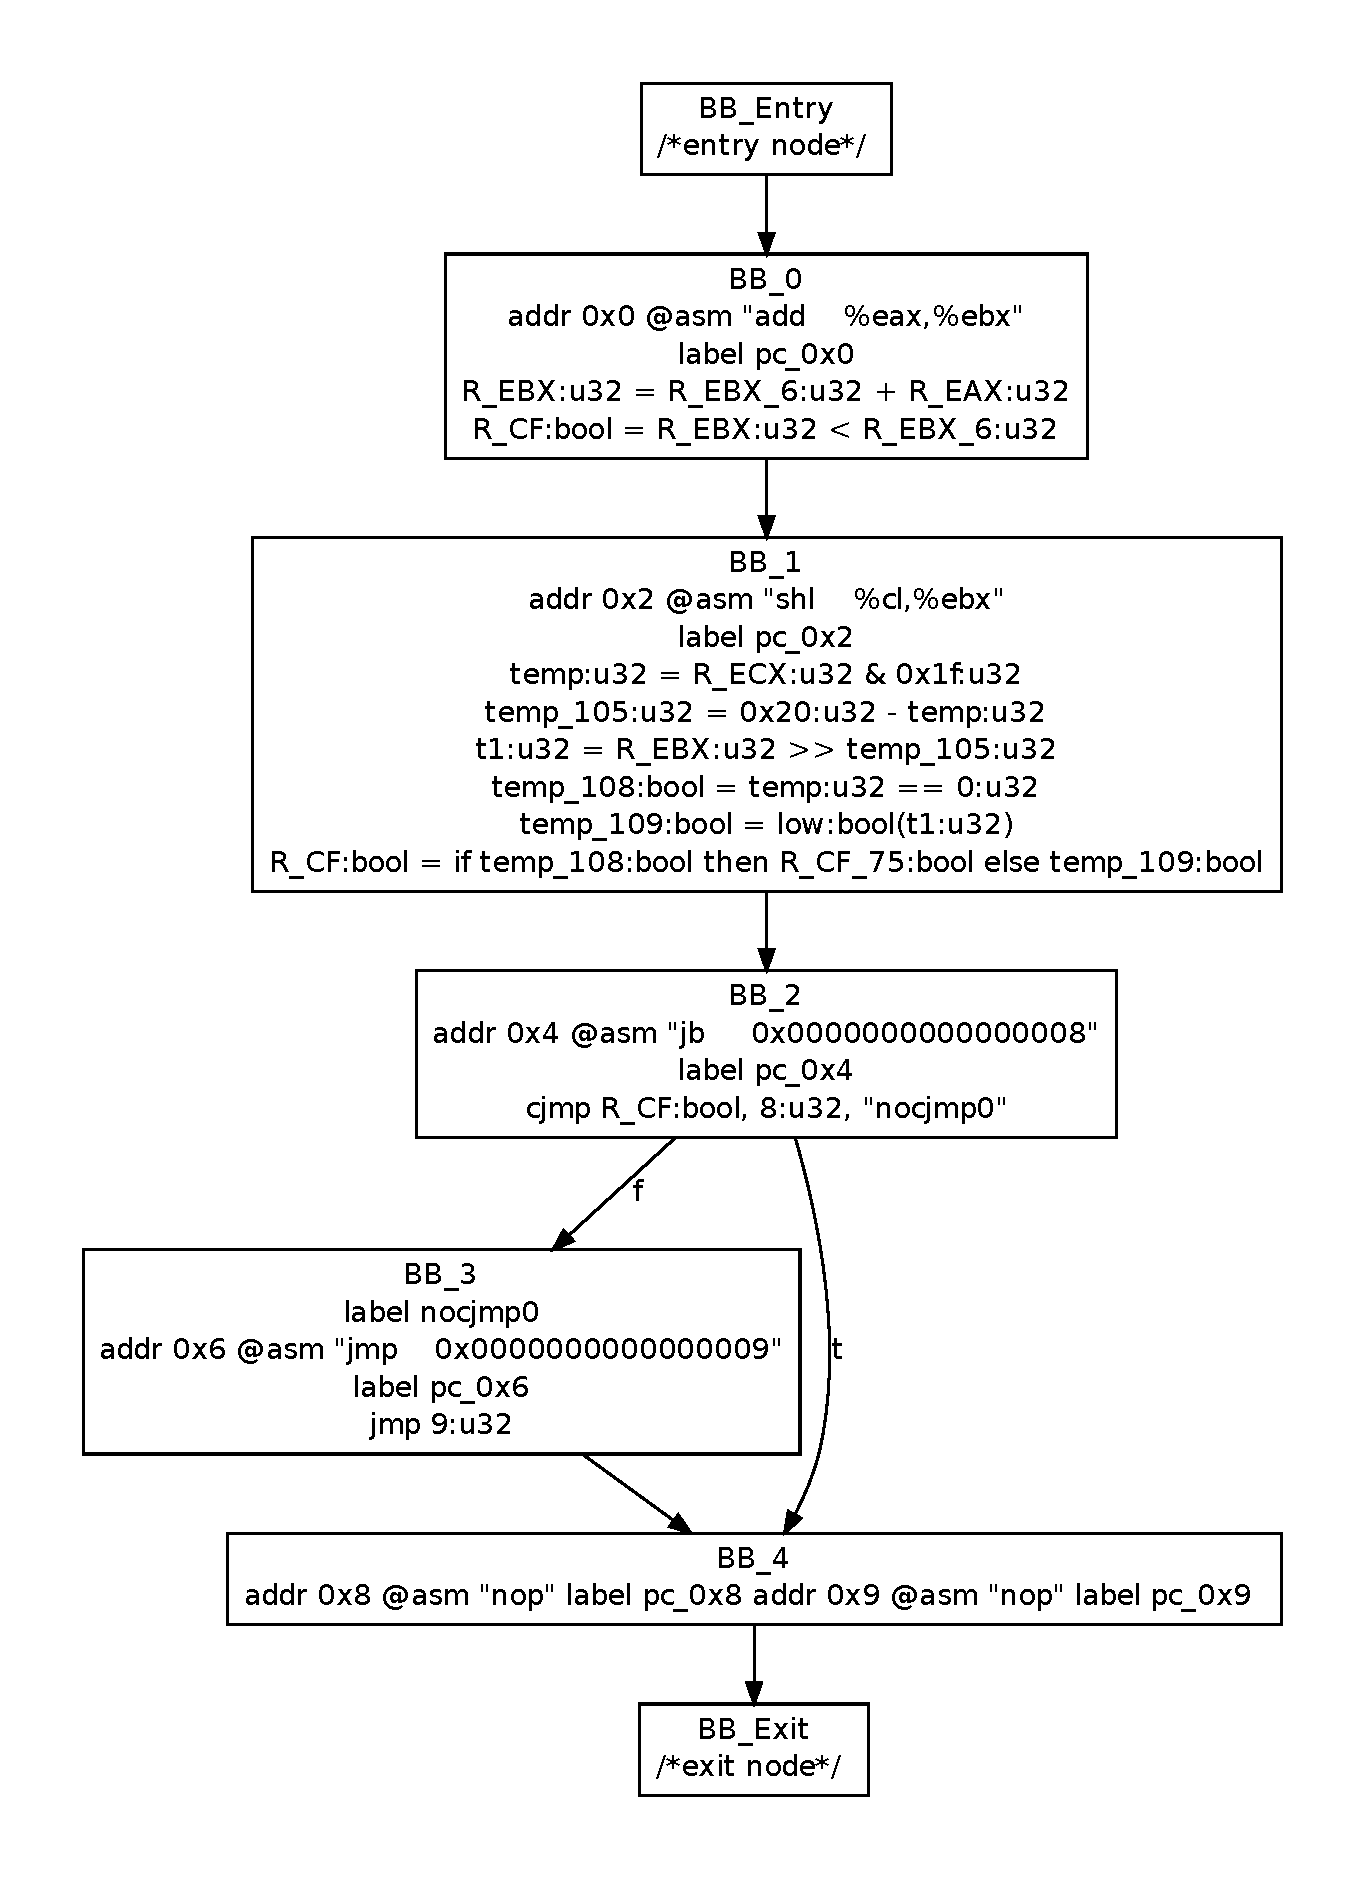
\includegraphics[height=.9\textheight]{chap-examples/cfg_simp.pdf}
  \end{center}
  \caption{Example Simplified CFG}
  \label{fig:cfgsimp}
\end{figure}
\FloatBarrier

\subsection{Verification Conditions}

Let's say we want to know if we can take the jump at address four.  We
can test this in BAP by using verification conditions (VCs).  To do
this, we need to add a helper variable to the IL that represents
success.  We can do this by setting the goal variable to false at the
beginning of the program, and setting it to true after the branch is
taken.  Below is the modified IL that does this.

\verbatiminput{chap-examples/basic_mod.il}

To see if we take the jump, we can use topredicate with the post
condition \cmdline{goal}: \cmdline{topredicate -q -il basic\_mod.il
  -stp-out /tmp/f -post goal -solve}.  This will create a VC, and then solve it
using the stp solver.  We got
\begin{verbatim}
R_ECX_7 -> 0x3
R_EAX_5 -> 0x20000000
R_EBX_6 -> 0
\end{verbatim}
as a satisfying answer. Sure enough, $0x0 + 0x20000000 = 0x20000000$
and $0x20000000 << 0x3$ sets the carry flag, so the program would take the jump.
